\documentclass{beamer}
\usetheme{Frankfurt}
\usetheme{CambridgeUS}
\usefonttheme{structuresmallcapsserif}
\usefonttheme{serif}
\setbeamertemplate{background canvas}[vertical shading][bottom=white,top=white]   
\setbeamercolor{math text}{fg=black!10!blue}
\setbeamercolor{block title}{bg=blue!40!white, fg=black}
\setbeamertemplate{navigation symbols}{}
\setbeamerfont{frametitle}{size=\normalsize}
\useoutertheme{mathASUlogo}
%\setbeamertemplate{enumerate items}[default]

\usepackage[utf8]{inputenc}
\usepackage[spanish]{babel}
\usepackage{amsmath}
\usepackage{amsfonts}
\usepackage{amssymb}
\usepackage{graphicx}
\usepackage{color}
\usepackage{listings}
\usepackage{hyperref}
\usepackage{wasysym}
\usepackage{alltt}
\usepackage{algorithmic}
\usepackage{cancel}
\usepackage{tikz}
\usetikzlibrary{arrows,backgrounds}
\tikzstyle{block}=[draw opacity=0.7,line width=1.4cm]

\graphicspath{{./Figuras/}{../Figuras/}{./}}
%\graphicspath{{./Figuras/}{../GGMC_2019/Figuras/}}

\definecolor{light-gray}{gray}{0.99}
\definecolor{light-blue}{rgb}{0.90,0.90,0.98}
\definecolor{light-yellow}{rgb}{0.95,0.95,0.10}
\definecolor{dark-green}{rgb}{0.10,0.50,0.10}

\definecolor{links}{rgb}{0.05,0.05,0.95}
\hypersetup{colorlinks,linkcolor=,urlcolor=links}

%%%%%%%%%%%%%%%%%%%%%%%%%%%%%% User specified LaTeX commands.
\newcommand{\Vector}[1]{{\underline{\mathbf{#1}}}}
\newcommand{\Tensor}[1]{{\underline{\underline{\mathbf{#1}}}}}
%%%%%%%%%%%%%%%%%%%%%%%%%%%%%%
% Definimos el punto decimal.
\spanishdecimal{.}
%%%%%%%%%%%%%%%%%%%%%%%%%%%%%%

%Global Background must be put in preamble
%\usebackgroundtemplate%
%{%
%$$\includegraphics[width=0.5\paperwidth]{python-logo}$$%
%}

% the beginning of each subsection:
\AtBeginSection[]
{
	\begin{frame}<beamer>{Contenido}
	\tableofcontents[currentsection]
\end{frame}
}

\title[GeoMaC]{Geof\'isica Matem\'atica y Computacional \\
%\textcolor{Lured}{\footnotesize{... }}\\
%\textcolor{Lured}{\footnotesize{...}}
}   
\author[\copyright LMCS, IGEF--UNAM]{Luis M. de la Cruz Salas} 
\institute[UNAM] 
{ 
{\small{Departamento de Recursos Naturales}} \\
\vspace{0.15cm}
{\small{Instituto de Geof\'isica}} \\ 
\vspace{0.15cm}
{\small{Universidad Nacional Aut\'onoma de M\'exico}} \\
\vspace{0.15cm}

\includegraphics[height=.85cm]{unamlogo.png} 
}

\date{\textcolor{Lured}{\footnotesize{Semestre 2021-I}}}

\subtitle{\textcolor{Lured}{Diferencias Finitas: Problemas estacionarios \\ Calibración }}

% To uncover everything in a step-wise fashion:
%\beamerdefaultoverlayspecification{<+->}


\begin{document}
	
\begin{frame}
\titlepage
\end{frame}

%\begin{frame}{Contenido}
%\tableofcontents
%\end{frame}

\lstset{language=python}
\lstset{keywordstyle=\color{blue}}
%\lstset{backgroundcolor=\color{darkgray}}
\lstset{basicstyle=\tiny}
%\lstset{emph={File,interactive,UnitSquare,Expression,FacetNormal,VariationalProblem,ds,grad,inner,dx,vector,solve,assemble,apply,assign,plot,TestFunction,TrialFunction,Function,Rectangle,FunctionSpace,Constant,DirichletBC,interpolate},emphstyle=\color{red}}
\lstset{commentstyle=\textit}
\lstset{frame=trbl}


\begin{frame}{Calibración 1}

\begin{exampleblock}{Conducción en 1D con condiciones de tipo Dirichlet}

\begin{eqnarray*}
\frac{d^2 u(x)}{d x^2} & = & -\omega ^2 u(x) \,\,\,\,\, x \in [0,1] \\
u(0) & = & 1 \\
u(1) & = & 1
\end{eqnarray*}

Soluci\'on anal\'itica:
$\displaystyle
\boxed{u(x) = \frac{1-\cos(\omega)}{\sin(\omega)} \sin(f x) + b\cos(f x)}
$

\strut

donde $\omega$ = constante. 

\strut

{\footnotesize \textbf{Observación}: La ecuación también se puede escribir como:
\[
\frac{d^2 u(x)}{d x^2} + \omega ^2 u(x) = 0
\]}
\end{exampleblock}

\end{frame}


\begin{frame}{Calibración 2}

\begin{exampleblock}{Poisson en 1D con una condici\'on de tipo Neumman}
	
\begin{eqnarray*}
	\frac{d^2 u(x)}{d x^2} & = & e^x \,\,\,\,\, x \in [0,1] \\
	\frac{du}{d n}(0) & = & 0 \\
	u(1) & = & 3
\end{eqnarray*}
	
Soluci\'on anal\'itica:
$\displaystyle \boxed{u(x) = e^x - x - e + 4} $

\end{exampleblock}

\end{frame}

\begin{frame}{Ecuaci\'on de Poisson 1D : BC Neumman I}

$$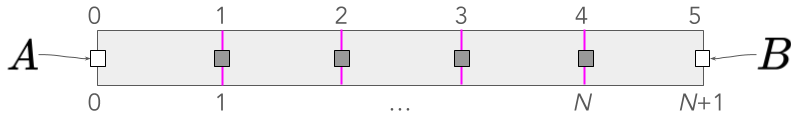
\includegraphics[scale=0.30]{ModCon06.png}$$
	
\begin{footnotesize}
\begin{columns}
	\begin{column}{0.45\textwidth}
		$ u_0  = A $
		
		$u_{0} - 2 u_{1} + u_{2} = r^{-1} f_1$ 
		
		$\Rightarrow \boxed{-2 u_{1} + u_{2} = r^{-1} f_1 - A}$
	\end{column}
	\begin{column}{0.5\textwidth}
		$\left.\displaystyle \frac{\partial u}{\partial n}\right|_{N+1}  = B \Longrightarrow \boxed{u_{N+1} - u_{N} = h B}$  
		
	\end{column}
\end{columns}
	
\strut
	
\[
\Longrightarrow
\underbrace{
	\left[
	\begin{matrix}
	-2 & 1 & 0  & \dots & 0 & 0  \\
	1 & -2 & 1  & \dots & 0 & 0 \\
	\vdots & \ddots & \ddots & \ddots & \vdots & \vdots \\
	0 & \dots & 1 & -2 & 1 & 0 \\
	0 & \dots & 0 & 1 & -2 & 1 \\
	0 & \dots & 0 & 0 & -1 & 1        
	\end{matrix}
	\right] 
}_{(N+1) \times (N+1)}
\left[
\begin{matrix}
u_1 \\ u_2 \\ \vdots \\ u_{N-1} \\ u_N \\ u_{N+1}
\end{matrix}
\right]= 
\frac{1}{r}\left[
\begin{matrix}
f_1 \\ f_2 \\ \vdots \\ f_{N-1} \\ f_N \\ 0
\end{matrix}
\right] +
\left[
\begin{matrix}
-A \\ 0 \\  \vdots \\ 0 \\ 0 \\ hB
\end{matrix}
\right]
\]
\end{footnotesize}

\end{frame}

\begin{frame}{Ecuaci\'on de Poisson 1D : BC Neumman II}

$$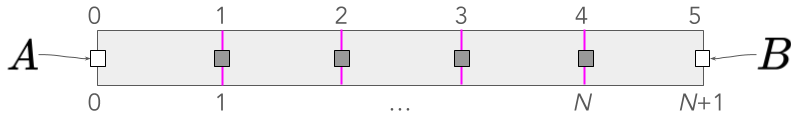
\includegraphics[scale=0.30]{ModCon06.png}$$

\begin{footnotesize}
\begin{columns}
	\begin{column}{0.45\textwidth}
		$ u_0  = A $
		
		$u_{0} - 2 u_{1} + u_{2} = r^{-1} f_1$ 
		
		$\Rightarrow \boxed{-2 u_{1} + u_{2} = r^{-1} f_1 - A}$
	\end{column}
	\begin{column}{0.5\textwidth}
		$\left.\displaystyle \frac{\partial u}{\partial n}\right|_{N+1}  = B \Longrightarrow \boxed{u_{N+1} = h B + u_{N}}$  
		
		$u_{N-1} - 2 u_{N} + u_{N+1} = r^{-1} f_N$
		
		$\Rightarrow \boxed{u_{N-1} - u_{N} = r^{-1} f_N - hB}$
	\end{column}
\end{columns}

\vspace{0.25cm}

\[
\Longrightarrow
\underbrace{
	\left[
	\begin{matrix}
	-2 & 1 & 0 & 0 & \dots & 0  \\
	1 & -2 & 1 & 0 & \dots & 0  \\
	0 & 1 & -2 & 1 & \dots & 0  \\
	\vdots & \ddots & \ddots & \ddots & \ddots & \vdots \\
	0 & 0 & 0 & 1 & -2 & 1   \\
	0 & 0 & 0 & 0 & 1 & -1    
	\end{matrix}
	\right] }_{N \times N}
\left[
\begin{matrix}
u_1 \\ u_2 \\ u_3 \\ \vdots \\ u_{N-1} \\ u_N
\end{matrix}
\right]= 
\frac{1}{r} \left[
\begin{matrix}
f_1 \\ f_2 \\ f_3 \\ \vdots \\ f_{N-1} \\ f_N
\end{matrix}
\right] +
\left[
\begin{matrix}
-A \\ 0 \\ 0 \\ \vdots \\ 0 \\ -hB
\end{matrix}
\right]
\]

\end{footnotesize}

\end{frame}

\begin{frame}{Ecuaci\'on de Poisson 1D : BC Neumman III}

$$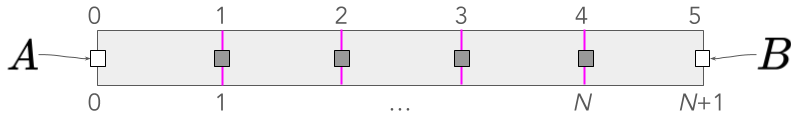
\includegraphics[scale=0.30]{ModCon06.png}$$

\begin{footnotesize}
\begin{columns}
\begin{column}{0.40\textwidth}
	$ u_0  = A $.
	
	$u_{0} - 2 u_{1} + u_{2} = r^{-1} f_1$ 
	
	$\Rightarrow \boxed{-2 u_{1} + u_{2} = r^{-1} f_1 - A}$
\end{column}
\begin{column}{0.6\textwidth}
	$\left.\displaystyle \frac{\partial u}{\partial n}\right|_{N+1}  = 
	\boxed{\frac{1}{h}\left( \frac{3}{2} u_{N+1} - 2 u_{N} + \frac{1}{2} u_{N-1} \right) = B}$
	
\end{column}
\end{columns}

\vspace{0.25cm}

\[
\Longrightarrow
\underbrace{
\left[
\begin{matrix}
-2 & 1 & 0  & \dots & 0 & 0  \\
1 & -2 & 1  & \dots & 0 & 0 \\
\vdots & \ddots & \ddots & \ddots & \vdots & \vdots \\
0 & \dots & 1 & -2 & 1 & 0 \\
0 & \dots & 0 & 1 & -2 & 1 \\
0 & \dots & 0 & \frac{1}{2} & -2 & \frac{3}{2}        
\end{matrix}
\right] 
}_{(N+1) \times (N+1)}
\left[
\begin{matrix}
u_1 \\ u_2 \\ \vdots \\ u_{N-1} \\ u_N \\ u_{N+1}
\end{matrix}
\right]= 
\frac{1}{r} \left[
\begin{matrix}
f_1 \\ f_2 \\ \vdots \\ f_{N-1} \\ f_N \\ 0
\end{matrix}
\right] +
\left[
\begin{matrix}
-A \\ 0 \\  \vdots \\ 0 \\ 0 \\ hB
\end{matrix}
\right]
\]


\end{footnotesize}

\end{frame}

\begin{frame}{Ecuaci\'on de Poisson 1D : BC Neumman IV}

$$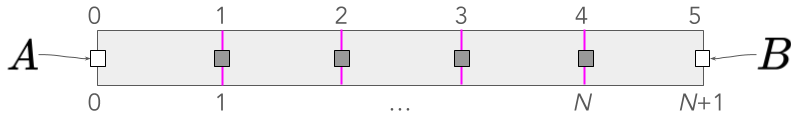
\includegraphics[scale=0.30]{ModCon06.png}$$

\begin{footnotesize}
\begin{columns}
\begin{column}{0.40\textwidth}
$ u_0  = A $.

$u_{0} - 2 u_{1} + u_{2} = r^{-1} f_1$ 

$\Rightarrow \boxed{-2 u_{1} + u_{2} = r^{-1} f_1 - A}$
\end{column}
\begin{column}{0.6\textwidth}
$u_{N} - 2u_{N+1} + u_{N+2} = r^{-1} f_{N+1}$

$\left.\displaystyle \frac{\partial u}{\partial n}\right|_{N+1}  = 
\frac{1}{2h}\left( u_{N+2} - u_{N} \right) = B$

$\Longrightarrow \boxed{u_{N} - u_{N+1} = \frac{1}{2r} f_{N+1} - hB}$
\end{column}
\end{columns}

%\vspace{0.25cm}

\[
\Longrightarrow
\underbrace{
\left[
\begin{matrix}
-2 & 1 & 0  & \dots & 0 & 0  \\
1 & -2 & 1  & \dots & 0 & 0 \\
\vdots & \ddots & \ddots & \ddots & \vdots & \vdots \\
0 & \dots & 1 & -2 & 1 & 0 \\
0 & \dots & 0 & 1 & -2 & 1 \\
0 & \dots & 0 & 0 & 1 & -1        
\end{matrix}
\right] 
}_{(N+1) \times (N+1)}
\left[
\begin{matrix}
u_1 \\ u_2 \\ \vdots \\ u_{N-1} \\ u_N \\ u_{N+1}
\end{matrix}
\right]= 
\frac{1}{r} \left[
\begin{matrix}
f_1 \\ f_2 \\ \vdots \\ f_{N-1} \\ f_N \\ f_{N+1}/2
\end{matrix}
\right] +
\left[
\begin{matrix}
-A \\ 0 \\  \vdots \\ 0 \\ 0 \\ -hB
\end{matrix}
\right]
\]

\end{footnotesize}

\end{frame}

\begin{frame}{Medici\'on del error}

\begin{itemize}
\item Si $\hat{u}(x)$ representa la soluci\'on exacta del problema, definimos el error en el punto $x_i$ de la aproximaci\'on como $E_i = u(x_i) - \hat{u}(x_i)$. 

\item El vector $\Vector{E} = (E_0, E_1, \dots, E_{N+1})$ representa el error en todos los puntos de la malla. La magnitud de este vector debe darnos el error global de la aproximaci\'on. 

\item Se puede usar cualquier norma:

\begin{itemize}
\item Norma infinito: $ \displaystyle
|| E ||_\infty = \max\limits_{1 \leq i \leq N}|E_i| = \max\limits_{1 \leq i \leq N} |u(x_i) - \hat{u}(x_i) |$

\item Norma uno:
\[
||E||_1 = h \sum\limits_{i=1}^{N} |E_i|
\]

\item Norma Euclideana:
\[
||E||_2 = \left(h \sum\limits_{i=1}^{N} |E_i|^2 \right)^{1/2}
\]
\end{itemize}

\end{itemize}

\end{frame}

\begin{frame}{Calibración 3}

\begin{exampleblock}{Ecuación de Poisson, conductividad no constante}

{\footnotesize 	
%|sin(4 \pi x)|

\begin{columns}
\begin{column}{0.5\textwidth}
\begin{equation}\label{eq:poisson1}
\dfrac{d}{d x} \left(\kappa \dfrac{d u}{d x} \right) = f \quad \text{con} \quad \kappa = \kappa(x)
\end{equation}
\end{column}
\begin{column}{0.5\textwidth}
$$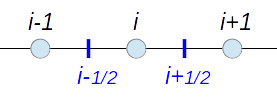
\includegraphics[scale=0.4]{malla1D_DF_Centrales.png}$$
\end{column}
\end{columns}

Definimos $\displaystyle g = \kappa \dfrac{d u}{d x}$ por lo tanto $\displaystyle \dfrac{d}{d x} \left(\kappa \dfrac{d u}{d x} \right) = \dfrac{d g}{d x}$:
	
	\begin{equation}\label{eq:poisson2}
	\dfrac{d g}{d x} \Big|_{i} = \dfrac{g_{i+\frac{1}{2}} - g_{i-\frac{1}{2}}}{h} =
	\dfrac{\left[\kappa \frac{du}{dx}\right]_{i+\frac{1}{2}} - \left[\kappa \frac{du}{dx}\right]_{i-\frac{1}{2}}}{h}
	\end{equation}
	
	\begin{equation}\label{eq:poisson3}
	\left[\kappa \frac{du}{dx}\right]_{i+\frac{1}{2}} = 
	\kappa_{i+\frac{1}{2}} \left[\dfrac{u_{i+1}-u_{i}}{h}\right] =
	\dfrac{1}{h}\left[\kappa_{i+\frac{1}{2}} u_{i+1} - \kappa_{i+\frac{1}{2}} u_{i}\right]
	\end{equation}
	
	\begin{equation}\label{eq:poisson4}
	\left[\kappa \frac{du}{dx}\right]_{i-\frac{1}{2}} = 
	\kappa_{i-\frac{1}{2}} \left[\dfrac{u_{i}-u_{i-1}}{h}\right] =
	\dfrac{1}{h}\left[\kappa_{i-\frac{1}{2}} u_{i} - \kappa_{i-\frac{1}{2}} u_{i-1}\right]
	\end{equation}
}

\end{exampleblock}

\end{frame}

\begin{frame}{Calibración 3}

\begin{exampleblock}{Ecuación de Poisson, conductividad no constante}
{\footnotesize 

Usando \eqref{eq:poisson2}, \eqref{eq:poisson3} y \eqref{eq:poisson4} en \eqref{eq:poisson1}:

\begin{equation}
\dfrac{1}{h^2} \left[
\kappa_{i+\frac{1}{2}} u_{i+1} - 
(\kappa_{i+\frac{1}{2}} + \kappa_{i-\frac{1}{2}}) u_{i} +
\kappa_{i-\frac{1}{2}} u_{i-1}
\right] = f_i
\end{equation}

Condiciones de frontera tipo Dirichlet: 
%
\[
\begin{array}{ccccc}
i = 1 & \Longrightarrow &
\kappa_{1+\frac{1}{2}} u_{2} - 
(\kappa_{1+\frac{1}{2}} + \kappa_{1-\frac{1}{2}}) u_{1} & = & h^2 f_1 - \kappa_{1-\frac{1}{2}} u_{0} \\ \\
i = N & \Longrightarrow &
- (\kappa_{N+\frac{1}{2}} + \kappa_{N-\frac{1}{2}}) u_{N} +
\kappa_{N-\frac{1}{2}} u_{N-1} & = & h^2 f_N - \kappa_{N+\frac{1}{2}} u_{N+1}
\end{array}
\]

\noindent
Donde $\kappa_{i+\frac{1}{2}}$ y $\kappa_{i-\frac{1}{2}}$ se pueden aproximar de varias maneras:

\[
\begin{array}{cccc}
\text{Promedio aritmético: } &
\kappa_{i+\frac{1}{2}} = \dfrac{ \kappa_{i+1} + \kappa_{i}}{2} & \text{ y } &
\kappa_{i-\frac{1}{2}} = \dfrac{ \kappa_{i-1} + \kappa_{i}}{2} \\
\text{Promedio geométrico: } &
\kappa_{i+\frac{1}{2}} = \dfrac{ \kappa_{i+1} + \kappa_{i}}{2} & \text{ y } &
\kappa_{i-\frac{1}{2}} = \dfrac{ \kappa_{i-1} + \kappa_{i}}{2} 
\end{array}
\]

}
\end{exampleblock}

\end{frame}


\begin{frame}[fragile]{Calibración 3}

\begin{exampleblock}{Ecuación de Poisson, conductividad no constante}


{\footnotesize 
$a = 0, \,\, b = 1, \,\, N = 50 (h = 0.0196078), \,\, A = 2.0, \,\, B = 1.0, \,\, \kappa = |sin(4 \pi x)|$
}
\begin{columns}
\begin{column}{0.5\textwidth}
$$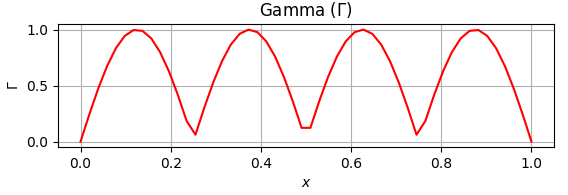
\includegraphics[width=6cm]{gamma.png}$$
\end{column}
\begin{column}{0.5\textwidth}  %%<--- here			
$$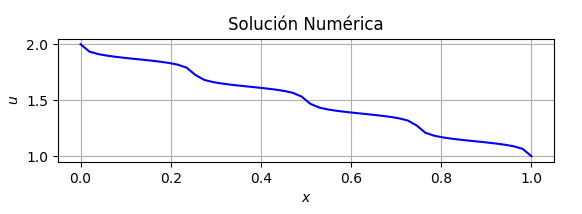
\includegraphics[width=6cm]{solucion02.png}$$
\end{column}
\end{columns}

{\footnotesize 
$a = 0, \,\, b = 1, \,\, N = 50 (h = 0.0196078), \,\, A = 2.0, \,\, B = 1.0, \,\, \kappa = \texttt{random(x)}$
}
\begin{columns}
\begin{column}{0.5\textwidth}
$$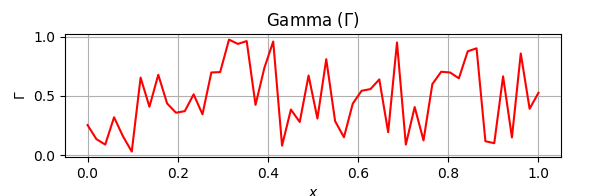
\includegraphics[width=6cm]{gamma3.png}$$
\end{column}
\begin{column}{0.5\textwidth}  %%<--- here			
$$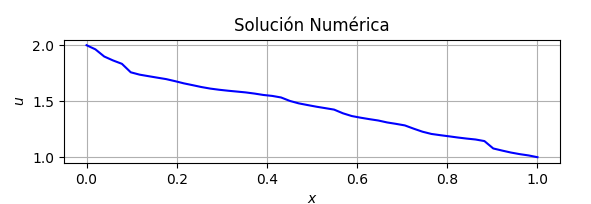
\includegraphics[width=6cm]{solucion03.png}$$
\end{column}
\end{columns}

{\footnotesize 
\begin{flushright}
\fcolorbox{blue}{light-blue}{\textcolor{dark-green}{\texttt{>python 1D\_Poisson\_02.py}}}
\end{flushright}
}

\end{exampleblock}

\end{frame}


\begin{frame}{Ecuaci\'on de Poisson 2D}

\begin{columns}
	\begin{column}{0.60\textwidth}
		\begin{small}
			\[
			\frac{\partial^2 u}{\partial x^2} + \frac{\partial^2 u}{\partial y^2} = f
			\]
			%
			\begin{eqnarray*}
				\frac{\partial^2 u}{\partial x^2}\Big|_{i,j} \approx \frac{u_{i+1,j} - 2 u_{i,j} + u_{i-1,j}}{h_x^2}; \\
				\frac{\partial^2 u}{\partial y^2}\Big|_{i,j} \approx \frac{u_{i,j+1} - 2 u_{i,j} + u_{i,j-1}}{h_y^2}.
			\end{eqnarray*}
			
			%Donde $h_x = L_x / (\textsf{N}_x + \textsf{1})$ y $h_y = L_y / (\textsf{N}_y + \textsf{1})$. 
		\end{small}
	\end{column}
	\begin{column}{0.40\textwidth}
		$$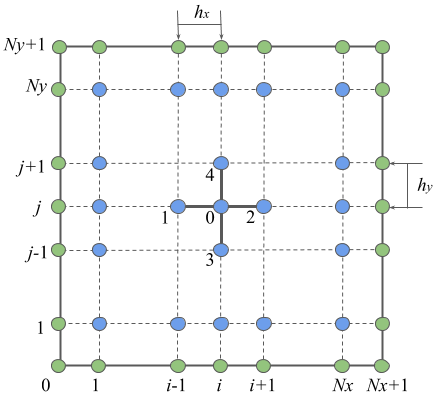
\includegraphics[scale=0.28]{malla2D_DF}$$
	\end{column}
\end{columns}

\begin{small}
	Donde $h_x = L_x / (\textsf{N}_x + \textsf{1})$ y $h_y = L_y / (\textsf{N}_y + \textsf{1})$. 
	Cuando $h_x = h_y = h$ entonces:
	\[
	\boxed{-4u_{i,j} +  u_{i-1,j} + u_{i+1,j} + u_{i,j-1} + u_{i,j+1} = h^2 f_{i,j}}
	\]
	
	\textit{Stencil}:
	$0 \equiv (i,j)$; $1 \equiv (i-1,j)$; $2 \equiv (i+1,j)$; $3 \equiv (i,j-1)$; $4 \equiv (i,j+1)$.
	
\end{small}

\end{frame}


\begin{frame}{Matriz 2D : Pentadiagonales}

{\tiny \[
\left[
\begin{array}{cccc|cccc|ccc}
-4 & 1 & 0 & 0 &  1 & 0 & 0 & 0 & 0 & 0 & \dots\\
1 &-4 & 1 & 0 &  0 & 1 & 0 & 0 & 0 & 0 & \dots\\
0 & 1 &-4 & 1 &  0 & 0 & 1 & 0 & 0 & 0 & \dots\\
0 & 0 & 1 &-4 &  0 & 0 & 0 & 1 & 0 & 0 & \dots\\
\hline
1 & 0 & 0 & 0 & -4 & 1 & 0 & 0 & 1 & 0 & \dots\\
0 & 1 & 0 & 0 &  1 &-4 & 1 & 0 & 0 & 1 & \dots\\
0 & 0 & 1 & 0 &  0 & 1 &-4 & 1 & 0 & 0 & \dots\\
0 & 0 & 0 & 1 &  0 & 0 & 1 &-4 & 0 & 0 & \dots\\
\hline
0 & 0 & 0 & 0 &  1 & 0 & 0 & 0 &-4 & 1 & \dots\\
0 & 0 & 0 & 0 &  0 & 1 & 0 & 0 & 1 &-4 & \dots\\
0 & 0 & 0 & 0 &  0 & 0 & 1 & 0 & 0 & 1 & \dots\\
\vdots & \vdots & \vdots & \vdots & \vdots & \vdots & \vdots & \vdots & \vdots & \vdots & \ddots 
\end{array} \right]
\left[
\begin{array}{c}
u_{1,1} \\ u_{2,1} \\ u_{3,1}  \\ u_{4,1} \\ \hline
u_{1,2} \\ u_{2,2} \\ u_{3,2}  \\ u_{4,2} \\ \hline
u_{1,3} \\ u_{2,3} \\ u_{3,3}  \\ \vdots \\
\end{array}
\right] = 
\left[
\begin{array}{c}
f_{1,1} \\ f_{2,1} \\ f_{3,1}  \\ f_{4,1} \\ \hline
f_{1,2} \\ f_{2,2} \\ f_{3,2}  \\ f_{4,2} \\ \hline
f_{1,3} \\ f_{2,3} \\ f_{3,3}  \\ \vdots \\
\end{array}
\right]	
\]}

$$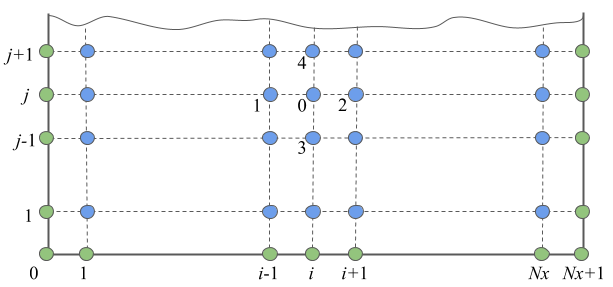
\includegraphics[scale=0.3]{malla2D_DF_R}$$
\end{frame}

\begin{frame}{Calibración 4}

\begin{exampleblock}{Ecuación de Laplace en 2D}

{\footnotesize
\begin{columns}
	\begin{column}{0.3\textwidth}
		$$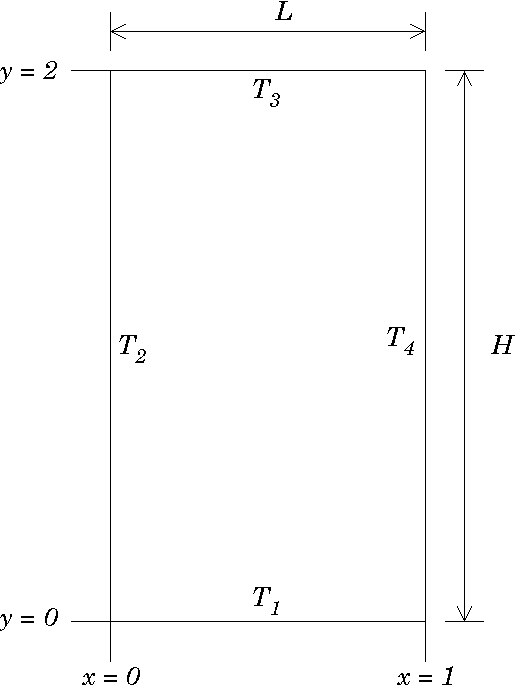
\includegraphics[width=3.5cm]{Hoffman.png}$$
	\end{column}
	\begin{column}{0.7\textwidth}
		\begin{eqnarray*}
			\nabla^2 T(\vec{x}) & = & 0 \,\,\,\,\, \text{para} \,\,\,\,\, \vec{x} \in [0,1] \times [0,2] \\
			T_1 & = & 100 \\
			T_2 & = & 0 \\
			T_3 & = & 0 \\
			T_4 & = & 0 
		\end{eqnarray*}
	
		Soluci\'on analítica: 
		
		$\displaystyle 
		\boxed{
		T(\vec{x}) = T_1 \left[ 
		2\sum_{n=1}^{\infty} \frac{1-(-1)^n}{n \pi} 
		\frac{\sinh \left( \frac{n \pi (H-y)}{L} \right)}
		{\sinh \left( \frac{n \pi H}{L} \right)} 
		\sin \left( \frac{n \pi x}{L} \right)
		\right]
		}
		$
	\end{column}
\end{columns}
}
\end{exampleblock}

\end{frame}

\begin{frame}{Ecuaci\'on de Poisson 2D: ¿Qué pasa cuando $hx \neq hy$ ?}

\begin{columns}
	\begin{column}{0.45\textwidth}
		\begin{small}
		\[
		-\nabla \cdot \left(\Tensor{\kappa} \nabla u \right) =  f
		\]
		\[
		\Tensor{\kappa} = 
		\left(\begin{array}{cc}
		\kappa_x & 0 \\
		0 & \kappa_y
		\end{array}\right)
		\]
		\[ \Longrightarrow
		-\left(\kappa_x \frac{\partial^2 u}{\partial x^2} + \kappa_y \frac{\partial^2 u}{\partial y^2}\right) = f
		\]
		\end{small}
	\end{column}
	\begin{column}{0.55\textwidth}
{\small 	
	\begin{eqnarray*}
		\kappa_x\frac{\partial^2 u}{\partial x^2}\Big|_{i,j} \approx \left(\kappa_x\right)_{i,j} \frac{u_{i+1,j} - 2 u_{i,j} + u_{i-1,j}}{h_x^2}; \\
		\kappa_y\frac{\partial^2 u}{\partial y^2}\Big|_{i,j} \approx \left(\kappa_x\right)_{i,j} \frac{u_{i,j+1} - 2 u_{i,j} + u_{i,j-1}}{h_y^2}.
	\end{eqnarray*}}
	\end{column}
\end{columns}

\begin{columns}
	\begin{column}{0.65\textwidth}
\begin{footnotesize}
	\[
	\boxed{A u_{i,j} + B u_{i-1,j} + C u_{i+1,j} + D u_{i,j-1} + E u_{i,j+1} = f_{i,j}}
	\]
	$\displaystyle A = -\left(\frac{2 \kappa_x}{h_x^2} + \frac{2 \kappa_y}{h_y^2}\right)_{i,j} = -(B + C + D + E)$;
	
	$\displaystyle B = \left(\frac{\kappa_x}{h_x^2}\right)_{i,j}$; 
	$\displaystyle C = \left(\frac{\kappa_x}{h_x^2}\right)_{i,j}$; 
	
	$\displaystyle D = \left(\frac{\kappa_y}{h_y^2}\right)_{i,j}$; 
	$\displaystyle E = \left(\frac{\kappa_y}{h_y^2}\right)_{i,j}$; 	
\end{footnotesize}
	\end{column}
	\begin{column}{0.35\textwidth}
		$$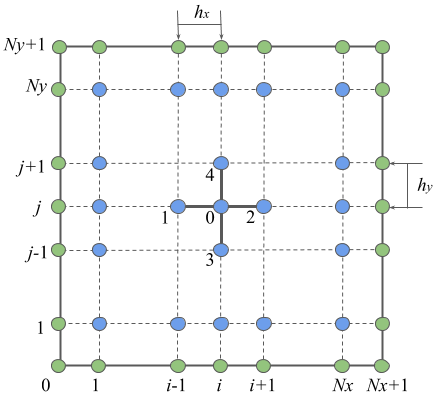
\includegraphics[scale=0.28]{malla2D_DF}$$
	\end{column}
\end{columns}

\end{frame}


\begin{frame}{Matriz 2D : Pentadiagonales}

{\tiny \[
	\left[
	\begin{array}{cccc|cccc|ccc}
	A & B & 0 & 0 & D & 0 & 0 & 0 & 0 & 0 & \dots\\
	C & A & B & 0 & 0 & D & 0 & 0 & 0 & 0 & \dots\\
	0 & C & A & B & 0 & 0 & D & 0 & 0 & 0 & \dots\\
	0 & 0 & C & A & 0 & 0 & 0 & D & 0 & 0 & \dots\\
	\hline
	E & 0 & 0 & 0 & A & B & 0 & 0 & D & 0 & \dots\\
	0 & E & 0 & 0 & C & A & B & 0 & 0 & D & \dots\\
	0 & 0 & E & 0 & 0 & C & A & B & 0 & 0 & \dots\\
	0 & 0 & 0 & E & 0 & 0 & C & A & 0 & 0 & \dots\\
	\hline
	0 & 0 & 0 & 0 &  E & 0 & 0 & 0 & A & B & \dots\\
	0 & 0 & 0 & 0 &  0 & E & 0 & 0 & C & A & \dots\\
	0 & 0 & 0 & 0 &  0 & 0 & E & 0 & 0 & C & \dots\\
	\vdots & \vdots & \vdots & \vdots & \vdots & \vdots & \vdots & \vdots & \vdots & \vdots & \ddots 
	\end{array} \right]
	\left[
	\begin{array}{c}
	u_{1,1} \\ u_{2,1} \\ u_{3,1}  \\ u_{4,1} \\ \hline
	u_{1,2} \\ u_{2,2} \\ u_{3,2}  \\ u_{4,2} \\ \hline
	u_{1,3} \\ u_{2,3} \\ u_{3,3}  \\ \vdots \\
	\end{array}
	\right] = 
	\left[
	\begin{array}{c}
	f_{1,1} \\ f_{2,1} \\ f_{3,1}  \\ f_{4,1} \\ \hline
	f_{1,2} \\ f_{2,2} \\ f_{3,2}  \\ f_{4,2} \\ \hline
	f_{1,3} \\ f_{2,3} \\ f_{3,3}  \\ \vdots \\
	\end{array}
	\right]	
	\]}

$$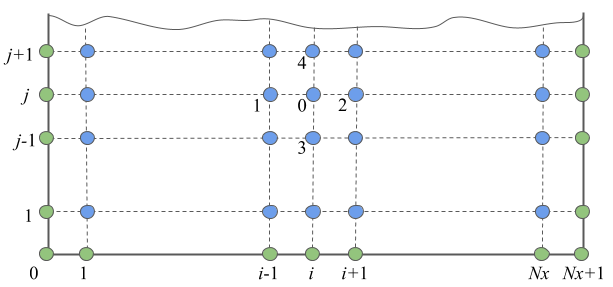
\includegraphics[scale=0.3]{malla2D_DF_R}$$
\end{frame}

\begin{frame}{Ecuaci\'on de Poisson 3D}

\begin{columns}
\begin{column}{0.70\textwidth}
\begin{small}
\[
\frac{\partial^2 u}{\partial x^2} + \frac{\partial^2 u}{\partial y^2} + \frac{\partial^2 u}{\partial z^2}= f
\]
%
\begin{eqnarray*}
\frac{\partial^2 u}{\partial x^2}\Big|_{i,j,k} & \approx & \frac{u_{i+1,j,k} - 2 u_{i,j,k} + u_{i-1,j,k}}{h_x^2} ; \\
\frac{\partial^2 u}{\partial y^2}\Big|_{i,j,k} & \approx & \frac{u_{i,j+1,k} - 2 u_{i,j,k} + u_{i,j-1,k}}{h_y^2} ; \\
\frac{\partial^2 u}{\partial z^2}\Big|_{i,j,k} & \approx & \frac{u_{i,j,k+1} - 2 u_{i,j,k} + u_{i,j,k-1}}{h_z^2} .
\end{eqnarray*} 
%
\end{small} 
\end{column}
\begin{column}{0.30\textwidth}
$$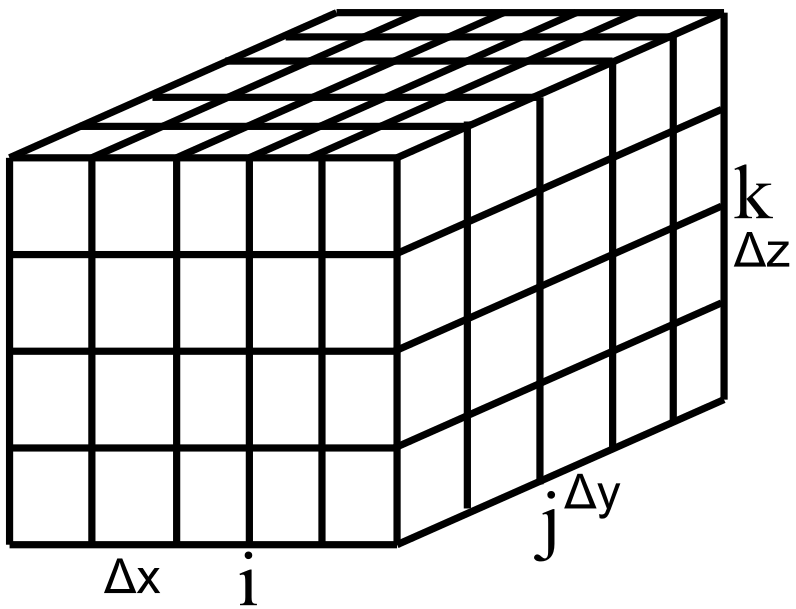
\includegraphics[scale=0.12]{malla3D_DF}$$
$$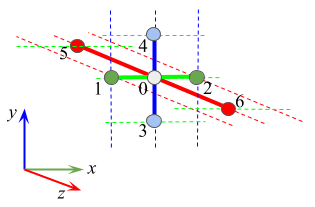
\includegraphics[scale=0.30]{stencil3D_DF}$$
\end{column}
\end{columns}

\begin{small}
Donde $h_x = L_x / (\textsf{N}_x + \textsf{1})$, $h_y = L_y / (\textsf{N}_y + \textsf{1})$ y $h_z = L_z / (\textsf{N}_z + \textsf{1})$. 
Cuando $h_x = h_y = h_z = h$ entonces:
\[
\boxed{-6u_{i,j,k} +  u_{i-1,j,k} + u_{i+1,j,k} + u_{i,j-1,k} + u_{i,j+1,k} + u_{i,j,k-1} + u_{i,j,k+1} = h^2 f_{i,j,k}}
\]
\end{small}

%\begin{tikzpicture}
%\draw[help lines,white] (0,0) grid (12,7);
%\end{tikzpicture}

\end{frame}

\begin{frame}{Matriz 3D : Heptadiagonales}

\begin{tiny}
\[
\left[
\begin{array}{ccc|ccc|ccc||ccc|ccc|cc}
-6 & 1 & 0 & 1 & 0 & 0 & 0 & 0 & 0 & 1 & 0 & 0 & 0 & 0 & 0 & 0 & \dots\\
1 &-6 & 1 & 0 & 1 & 0 & 0 & 0 & 0 & 0 & 1 & 0 & 0 & 0 & 0 & 0 & \dots\\
0 & 1 &-6 & 0 & 0 & 1 & 0 & 0 & 0 & 0 & 0 & 1 & 0 & 0 & 0 & 0 & \dots\\
\hline
1 & 0 & 0 &-6 & 1 & 0 & 1 & 0 & 0 & 0 & 0 & 0 & 1 & 0 & 0 & 0 & \dots\\
0 & 1 & 0 & 1 &-6 & 1 & 0 & 1 & 0 & 0 & 0 & 0 & 0 & 1 & 0 & 0 & \dots\\
0 & 0 & 1 & 0 & 1 &-6 & 0 & 0 & 1 & 0 & 0 & 0 & 0 & 0 & 1 & 0 & \dots\\
\hline
0 & 0 & 0 & 1 & 0 & 0 &-6 & 1 & 0 & 0 & 0 & 0 & 0 & 0 & 0 & 1 & \dots\\
0 & 0 & 0 & 0 & 1 & 0 & 1 &-6 & 1 & 0 & 0 & 0 & 0 & 0 & 0 & 0 & \dots\\
0 & 0 & 0 & 0 & 0 & 1 & 0 & 0 &-6 & 0 & 0 & 0 & 0 & 0 & 0 & 0 & \dots\\
\hline
\hline
1 & 0 & 0 & 0 & 0 & 0 & 0 & 0 & 0 &-6 & 1 & 0 & 1 & 0 & 0 & 0 & \dots\\
0 & 1 & 0 & 0 & 0 & 0 & 0 & 0 & 0 & 1 &-6 & 1 & 0 & 1 & 0 & 0 & \dots\\
0 & 0 & 1 & 0 & 0 & 0 & 0 & 0 & 0 &0 & 1 &-6 & 0 & 0 & 1 & 0 & \dots\\
\hline
0 & 0 & 0 & 1 & 0 & 0 & 0 & 0 & 0 & 1 & 0 & 0 &-6 &-1 & 0 & 1 & \dots\\
0 & 0 & 0 & 0 & 1 & 0 & 0 & 0 & 0 & 0 & 1 & 0 & 1 &-6 & 1 & 0 & \dots\\
0 & 0 & 0 & 0 & 0 & 1 & 0 & 0 & 0 & 0 & 0 & 1 & 0 & 1 &-6 & 0 & \dots\\
\vdots & \vdots & \vdots & \vdots & \vdots & \vdots & \vdots & \vdots & \vdots & \vdots 
& \vdots & \vdots & \vdots & \vdots & \vdots & \vdots
& \ddots 
\end{array} \right]
\]
\end{tiny}

\end{frame}



%{\footnotesize{
%\begin{itemize}
%\item Dominio
%\begin{columns}
%\begin{column}{0.3\textwidth}
%$$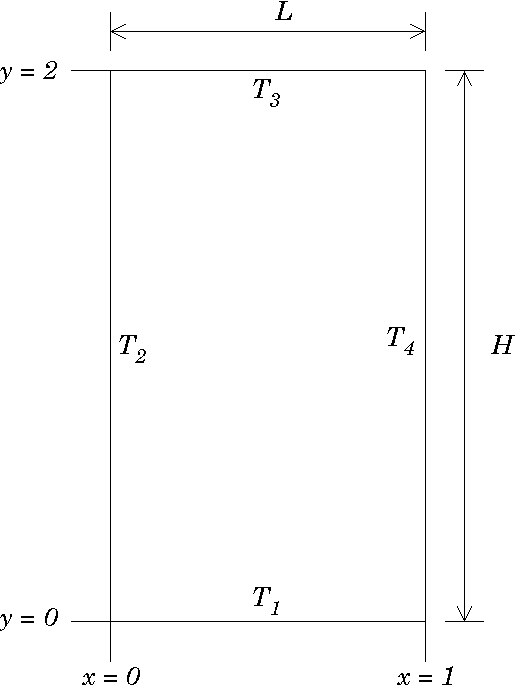
\includegraphics[width=2.5cm]{Hoffman.png}$$
%\end{column}
%\begin{column}{0.3\textwidth}
%$$\includegraphics[width=2.5cm]{HoffmanExact.png}$$
%\end{column}
%\begin{column}{0.3\textwidth}
%$$\includegraphics[width=3cm]{HoffmanExactS.png}$$
%\end{column}
%\end{columns}
%\item Ecuaci\'on y condiciones de frontera
%\begin{eqnarray*}
%\nabla^2 T(\Vector{x}) & = & 0 \,\,\,\,\, \text{para} \,\,\,\,\, \Vector{x} \in [0,1] \times [0,2] \\
%T_1 & = & 100; T_2 = T_3 = T_4 = 0 \,\,\,\,\, \text{(Cond. de frontera)} 
%\end{eqnarray*}
%\item Soluci\'on exacta: 
%$\displaystyle
%  T(\Vector{x}) = T_1 \left[ 
%    2\sum_{n=1}^{\infty} \frac{1-(-1)^n}{n \pi} 
%    \frac{\sinh \left( \frac{n \pi (H-y)}{L} \right)}
%    {\sinh \left( \frac{n \pi H}{L} \right)} 
%    \sin \left( \frac{n \pi x}{L} \right)
%    \right]
%$
%
%\end{itemize}
%}}







\end{document}
	